% Chapter 4 from the standard thesis template
%   that contains an adv. example table and figure.
\chapter{NULLABOR: AN R PACKAGE FOR VISUAL STATISTICAL INFERENCE}\label{ch:nullabor}
\vspace{0.8cm}
\begin{center}
\large{A paper to be submitted to \it{Journal of Statistical Software}.}

\large{Niladri Roy Chowdhury, Hadley Wickham, Dianne Cook, Heike Hofmann, \\
Mahbubul Majumder}\\
\end{center}

\section*{Abstract}

Statistical graphics play an important role in statistical analysis, model checking and data mining, but they have not been used for statistical inference. \cite{buja:2009} introduced protocols to allow inference to statistical graphics, which is also described in \cite{hadley:2010}. Later \cite{majumder:2013} describes a comparative study between classical inference methods and visual inference methods in a linear modeling setting. The recent developments in visual inference demands an open source platform which can be used to implement the visual methods. The R package \textbf{nullabor} provides methods of generating lineups automatically for different null generating methods and also construction of diagnostic plots to measure the quality of a lineup. In this paper we discuss the different tools in \textbf{nullabor} which helps to use visual inference easily.\\



\textbf{Keywords:} visual inference; lineup; null generating mechanisms

\newpage
\section{Introduction}\label{introduction}

Recent developments suggest that statistical graphics can be used to perform statistical inference. \cite{buja:2009} introduced protocols to allow inference to statistical graphics, which were later validated by \cite{majumder:2013}. The recent developments require a software package which would make the implementation of visual inference easier and automatic. \cite{buja:2009} describes two protocols which are known as the lineup protocol and the Rorschach protocol, which is also described in \cite{hadley:2010}. In the lineup protocol, the plot of the actual data is randomly placed in a set of null plots, These null plots are generated by a mechanism which is consistent with the null hypothesis. A human judge is shown the lineup and asked to identify the plot which is the most different or the plot which has the strongest structure. If the human judge can identify the plot of the actual data, we reject the null hypothesis. On the other hand, in the Rorschach protocol, all the plots are generated from the null distribution assuming that the null hypothesis is true. This protocol helps us to calibrate our eyes to the natural variability of the plots and hence reduce our sensitivity to structures which appear purely due to randomness. This package provides functions to implement these two protocols in different scenarios. 

The second part of the package introduces distance metrics. Distance metrics are used to measure distances between the plots in a lineup.  The null plots in a lineup may affect the decision of the human subjects since they base their decision on a finite number of null plots. Hence it is essential to measure the quality of the lineups by calculating the distances between the plot of the actual data and the null plots and the null plots among themselves. To compare several lineups, the distances obtained from a certain lineup are compared to the empirical distribution of the distances. 

This chapter is organized in the following way. Section \ref{null-gen} describes the different null generating mechanisms which are used to obtain the null plots in the lineup. The two protocols are described in Section \ref{protocols}. Section \ref{distance-metrics} discusses five different distance metrics. These are targeted for different varieties of data and plot types. Calculating different statistics from a lineup are described in the next section. Section \ref{select-bins} describes the procedure to select the optimal number of bins for binned distance. Finally Section \ref{distr} gives the method of obtaining and plotting the empirical distribution of the distance metrics.


\section{Null generating mechanisms}\label{null-gen}

The null plots in a lineup is obtained by a method which is consistent with the null hypothesis. Assuming that the null hypothesis is true, the null datasets are obtained, often, from the actual dataset. This process of generating the null datasets is called the null generating mechanism. There may be a variety of null generating mechanisms but the package provides
three different methods.

\subsection{Generate null data with a specific
distribution}\label{generate-null-data-with-a-specific-distribution}

The \texttt{"null\_dist"} function takes as input a variable name of the
data and a particular distribution. This variable in the data is
substituted by random generations of the particular distribution. The
different distributions include beta, cauchy, chi-squared, exponential,
f, gamma, geometric, log-normal, lognormal, logistic, negative binomial,
normal, poisson, t and weibull. A list of parameters of distribution can
also be provided as input. In case it is not provided,
\texttt{"fitdistr"} is used to estimate the parameters from the given
data. The function \texttt{"null\_dist"} returns a function that given
the data generates a null data set.

%\begin{Shaded}
%\begin{Highlighting}[]
%\KeywordTok{library}\NormalTok{(nullabor)}
%\KeywordTok{head}\NormalTok{(}\KeywordTok{null_dist}\NormalTok{(}\StringTok{"mpg"}\NormalTok{, }\DataTypeTok{dist =} \StringTok{"normal"}\NormalTok{)(mtcars))}
%\end{Highlighting}
%\end{Shaded}

\begin{verbatim}
> head(null_dist("mpg", dist = "normal")(mtcars))


                        mpg cyl disp  hp drat    wt  qsec vs am gear carb
Mazda RX4         29.536386   6  160 110 3.90 2.620 16.46  0  1    4    4
Mazda RX4 Wag     16.897772   6  160 110 3.90 2.875 17.02  0  1    4    4
Datsun 710        16.395593   4  108  93 3.85 2.320 18.61  1  1    4    1
Hornet 4 Drive     9.644472   6  258 110 3.08 3.215 19.44  1  0    3    1
Hornet Sportabout 11.456224   8  360 175 3.15 3.440 17.02  0  0    3    2
Valiant           25.417741   6  225 105 2.76 3.460 20.22  1  0    3    1
\end{verbatim}
%\begin{table}[ht]
%\centering
%\begin{tabular}{lrrrrrrrrrrr}
%  \hline
% & mpg & cyl & disp & hp & drat & wt & qsec & vs & am & gear & carb \\ 
%  \hline
%Mazda RX4 & 23.70 & 6 & 160 & 110 & 3.90 & 2.62 & 16.46 & 0 & 1 & 4 & 4 \\ 
%  Mazda RX4 Wag & 38.32 & 6 & 160 & 110 & 3.90 & 2.88 & 17.02 & 0 & 1 & 4 & 4 \\ 
%  Datsun 710 & 15.96 & 4 & 108 & 93 & 3.85 & 2.32 & 18.61 & 1 & 1 & 4 & 1 \\ 
%  Hornet 4 Drive & 23.55 & 6 & 258 & 110 & 3.08 & 3.21 & 19.44 & 1 & 0 & 3 & 1 \\ 
%  Hornet Sportabout & 14.97 & 8 & 360 & 175 & 3.15 & 3.44 & 17.02 & 0 & 0 & 3 & 2 \\ 
%  Valiant & 10.24 & 6 & 225 & 105 & 2.76 & 3.46 & 20.22 & 1 & 0 & 3 & 1 \\ 
%   \hline
%\end{tabular}
%\end{table}

%\begin{verbatim}
%                    mpg cyl disp  hp drat    wt  qsec vs am gear carb
% Mazda RX4         23.53   6  160 110 3.90 2.620 16.46  0  1    4    4
%## Mazda RX4 Wag     19.98   6  160 110 3.90 2.875 17.02  0  1    4    4
%## Datsun 710        30.34   4  108  93 3.85 2.320 18.61  1  1    4    1
%## Hornet 4 Drive    21.30   6  258 110 3.08 3.215 19.44  1  0    3    1
%## Hornet Sportabout 15.40   8  360 175 3.15 3.440 17.02  0  0    3    2
%## Valiant           17.15   6  225 105 2.76 3.460 20.22  1  0    3    1
%\end{verbatim}

\subsection{Generate null data by permuting a
variable}\label{generate-null-data-by-permuting-a-variable}

The \texttt{"null\_permute"} function takes as input a variable name of
the data. This variable is permuted to obtain the null dataset. The
function \texttt{"null\_dist"} returns a function that given the data
generates a null data set.

\begin{verbatim}
> head(null_permute("mpg")(mtcars))


                   mpg cyl disp  hp drat    wt  qsec vs am gear carb
Mazda RX4         19.7   6  160 110 3.90 2.620 16.46  0  1    4    4
Mazda RX4 Wag     21.4   6  160 110 3.90 2.875 17.02  0  1    4    4
Datsun 710        22.8   4  108  93 3.85 2.320 18.61  1  1    4    1
Hornet 4 Drive    30.4   6  258 110 3.08 3.215 19.44  1  0    3    1
Hornet Sportabout 21.0   8  360 175 3.15 3.440 17.02  0  0    3    2
Valiant           15.8   6  225 105 2.76 3.460 20.22  1  0    3    1
\end{verbatim}

%\begin{Shaded}
%\begin{Highlighting}[]
%\KeywordTok{head}\NormalTok{(}\KeywordTok{null_permute}\NormalTok{(}\StringTok{"mpg"}\NormalTok{)(mtcars))}
%\end{Highlighting}
%\end{Shaded}
%
%\begin{verbatim}
%##                    mpg cyl disp  hp drat    wt  qsec vs am gear carb
%## Mazda RX4         15.5   6  160 110 3.90 2.620 16.46  0  1    4    4
%## Mazda RX4 Wag     30.4   6  160 110 3.90 2.875 17.02  0  1    4    4
%## Datsun 710        26.0   4  108  93 3.85 2.320 18.61  1  1    4    1
%## Hornet 4 Drive    24.4   6  258 110 3.08 3.215 19.44  1  0    3    1
%## Hornet Sportabout 27.3   8  360 175 3.15 3.440 17.02  0  0    3    2
%## Valiant           10.4   6  225 105 2.76 3.460 20.22  1  0    3    1
%\end{verbatim}

\subsection{Generate null data with null residuals from a
model}\label{generate-null-data-with-null-residuals-from-a-model}

The function \texttt{"null\_lm"} takes as input a model specification
formula as defined by \texttt{"lm"} and method for generating null
residuals from the model. The three built in methods are `rotate',
`pboot' and `boot' defined by \texttt{"resid\_rotate"},
\texttt{"resid\_pboot"} and \texttt{"resid\_boot"} respectively. The
function returns a function which given the data generates a null
dataset.


%\begin{Shaded}
%\begin{Highlighting}[]
%\KeywordTok{head}\NormalTok{(}\KeywordTok{null_lm}\NormalTok{(wt~mpg, }\DataTypeTok{method =} \StringTok{'rotate'}\NormalTok{)(mtcars))}
%\end{Highlighting}
%\end{Shaded}
%
%\begin{verbatim}
%##                    mpg cyl disp  hp drat    wt  qsec vs am gear carb
%## Mazda RX4         21.0   6  160 110 3.90 3.355 16.46  0  1    4    4
%## Mazda RX4 Wag     21.0   6  160 110 3.90 2.940 17.02  0  1    4    4
%## Datsun 710        22.8   4  108  93 3.85 3.849 18.61  1  1    4    1
%## Hornet 4 Drive    21.4   6  258 110 3.08 3.770 19.44  1  0    3    1
%## Hornet Sportabout 18.7   8  360 175 3.15 3.650 17.02  0  0    3    2
%## Valiant           18.1   6  225 105 2.76 3.659 20.22  1  0    3    1
%##                    .resid .fitted
%## Mazda RX4          0.2659   3.089
%## Mazda RX4 Wag     -0.1493   3.089
%## Datsun 710         1.0137   2.836
%## Hornet 4 Drive     0.7370   3.033
%## Hornet Sportabout  0.2364   3.413
%## Valiant            0.1610   3.498
%\end{verbatim}

\begin{verbatim}
> head(null_lm(wt~mpg, method = 'rotate')(mtcars))


                   mpg cyl disp  hp drat       wt  qsec vs am gear carb
Mazda RX4         21.0   6  160 110 3.90 3.049169 16.46  0  1    4    4
Mazda RX4 Wag     21.0   6  160 110 3.90 2.634875 17.02  0  1    4    4
Datsun 710        22.8   4  108  93 3.85 2.917568 18.61  1  1    4    1
Hornet 4 Drive    21.4   6  258 110 3.08 3.126533 19.44  1  0    3    1
Hornet Sportabout 18.7   8  360 175 3.15 4.281755 17.02  0  0    3    2
Valiant           18.1   6  225 105 2.76 3.368690 20.22  1  0    3    1
                       .resid  .fitted
Mazda RX4         -0.03998504 3.089154
Mazda RX4 Wag     -0.45427860 3.089154
Datsun 710         0.08196630 2.835602
Hornet 4 Drive     0.09372421 3.032809
Hornet Sportabout  0.86861876 3.413136
Valiant           -0.12896315 3.497653
\end{verbatim}

\section{Protocols}\label{protocols}

\cite{buja:2009} introduces two protocols which bridges the gulf between traditional statistical inference and exploratory data analysis. The two protocols can be implemented in the following way:

\subsection{The lineup protocol}\label{the-lineup-protocol}

In this protocol, the plot of the real data is randomly embedded amongst
a set of null plots. The matrix of plots is known as a lineup. The null
plots are generated by a method consistent with the null hypothesis. The
lineup is shown to an observer. If the observer can pick the real data
as different from the others, this puts weight on the statistical
significance of the structure in the plot. The \texttt{"lineup"}
function returns a set of generated null datasets and the real data
embedded randomly among these null datasets. The method of null
generation should be provided in the lineup function for the null
datasets to be generated automatically along with the real dataset. The
users also have the option of generating the null datasets themselves
and providing them in the \texttt{"lineup"} function. The position of
the real dataset can be left missing and the function picks the position
at random. The function then returns the position as an encrypted code.
The encrypted code is copied and pasted on the R console to obtain the
true position of the plot.

%\begin{Shaded}
%\begin{Highlighting}[]
%\KeywordTok{library}\NormalTok{(nullabor)}
%\KeywordTok{head}\NormalTok{(}\KeywordTok{lineup}\NormalTok{(}\KeywordTok{null_permute}\NormalTok{(}\StringTok{"mpg"}\NormalTok{), mtcars), }\DecValTok{20}\NormalTok{)}
%\end{Highlighting}
%\end{Shaded}
%
%\begin{verbatim}
%## decrypt("jriG PHhH D5 QZXDhDZ5 Jl")
%\end{verbatim}
%
%\begin{verbatim}
%##     mpg cyl  disp  hp drat    wt  qsec vs am gear carb .sample
%## 1  14.7   6 160.0 110 3.90 2.620 16.46  0  1    4    4       1
%## 2  22.8   6 160.0 110 3.90 2.875 17.02  0  1    4    4       1
%## 3  21.4   4 108.0  93 3.85 2.320 18.61  1  1    4    1       1
%## 4  33.9   6 258.0 110 3.08 3.215 19.44  1  0    3    1       1
%## 5  16.4   8 360.0 175 3.15 3.440 17.02  0  0    3    2       1
%## 6  10.4   6 225.0 105 2.76 3.460 20.22  1  0    3    1       1
%## 7  15.0   8 360.0 245 3.21 3.570 15.84  0  0    3    4       1
%## 8  19.7   4 146.7  62 3.69 3.190 20.00  1  0    4    2       1
%## 9  32.4   4 140.8  95 3.92 3.150 22.90  1  0    4    2       1
%## 10 18.7   6 167.6 123 3.92 3.440 18.30  1  0    4    4       1
%## 11 14.3   6 167.6 123 3.92 3.440 18.90  1  0    4    4       1
%## 12 10.4   8 275.8 180 3.07 4.070 17.40  0  0    3    3       1
%## 13 17.8   8 275.8 180 3.07 3.730 17.60  0  0    3    3       1
%## 14 22.8   8 275.8 180 3.07 3.780 18.00  0  0    3    3       1
%## 15 26.0   8 472.0 205 2.93 5.250 17.98  0  0    3    4       1
%## 16 27.3   8 460.0 215 3.00 5.424 17.82  0  0    3    4       1
%## 17 19.2   8 440.0 230 3.23 5.345 17.42  0  0    3    4       1
%## 18 30.4   4  78.7  66 4.08 2.200 19.47  1  1    4    1       1
%## 19 13.3   4  75.7  52 4.93 1.615 18.52  1  1    4    2       1
%## 20 15.8   4  71.1  65 4.22 1.835 19.90  1  1    4    1       1
%\end{verbatim}

\begin{verbatim}
> head(lineup(null_permute("mpg"), mtcars), 20)


decrypt("jriG PHhH D5 QZXDhDZ5 Jf")
    mpg cyl  disp  hp drat    wt  qsec vs am gear carb .sample
1  15.8   6 160.0 110 3.90 2.620 16.46  0  1    4    4       1
2  16.4   6 160.0 110 3.90 2.875 17.02  0  1    4    4       1
3  21.4   4 108.0  93 3.85 2.320 18.61  1  1    4    1       1
4  30.4   6 258.0 110 3.08 3.215 19.44  1  0    3    1       1
5  17.8   8 360.0 175 3.15 3.440 17.02  0  0    3    2       1
6  18.7   6 225.0 105 2.76 3.460 20.22  1  0    3    1       1
7  19.2   8 360.0 245 3.21 3.570 15.84  0  0    3    4       1
8  10.4   4 146.7  62 3.69 3.190 20.00  1  0    4    2       1
9  21.0   4 140.8  95 3.92 3.150 22.90  1  0    4    2       1
10 27.3   6 167.6 123 3.92 3.440 18.30  1  0    4    4       1
11 15.5   6 167.6 123 3.92 3.440 18.90  1  0    4    4       1
12 15.2   8 275.8 180 3.07 4.070 17.40  0  0    3    3       1
13 18.1   8 275.8 180 3.07 3.730 17.60  0  0    3    3       1
14 21.0   8 275.8 180 3.07 3.780 18.00  0  0    3    3       1
15 15.2   8 472.0 205 2.93 5.250 17.98  0  0    3    4       1
16 22.8   8 460.0 215 3.00 5.424 17.82  0  0    3    4       1
17 14.3   8 440.0 230 3.23 5.345 17.42  0  0    3    4       1
18 21.4   4  78.7  66 4.08 2.200 19.47  1  1    4    1       1
19 10.4   4  75.7  52 4.93 1.615 18.52  1  1    4    2       1
20 21.5   4  71.1  65 4.22 1.835 19.90  1  1    4    1       1

\end{verbatim}

The lineup data can be then used to generate the lineup using
\textbf{ggplot2}. The lineup is shown to one or more observers who are
asked to identify the plot which is different. If the observer can
identify the plot of the real data correctly, we reject the null
hypothesis and conclude that the plot of the real data has stronger
structure than the null plots. 

%\begin{Shaded}
%\begin{Highlighting}[]
%\KeywordTok{qplot}\NormalTok{(mpg, wt, }\DataTypeTok{data =} \KeywordTok{lineup}\NormalTok{(}\KeywordTok{null_permute}\NormalTok{(}\StringTok{"mpg"}\NormalTok{), mtcars)) +}\StringTok{ }\KeywordTok{facet_wrap}\NormalTok{(~}\StringTok{ }\NormalTok{.sample)}
%\end{Highlighting}
%\end{Shaded}
%
%\begin{verbatim}
%## decrypt("jriG PHhH D5 QZXDhDZ5 4")
%\end{verbatim}

\begin{verbatim}
> qplot(mpg, wt, data = lineup(null_permute("mpg"), mtcars)) + facet_wrap(~ .sample)

decrypt("jriG PHhH D5 QZXDhDZ5 l")
\end{verbatim}

Figure \ref{lineup-ex} is an example of a lineup plot where the plot of the actual data is embedded into nineteen null plots. The null plots are obtained by permuting the variable ``mpg'' while keeping the other variables fixed. The position of the actual plot is not known to the user. It can be obtained by copying the output in the R console. Hence the user can also act as a human judge. 

\begin{figure*}[hbtp]
\begin{center}
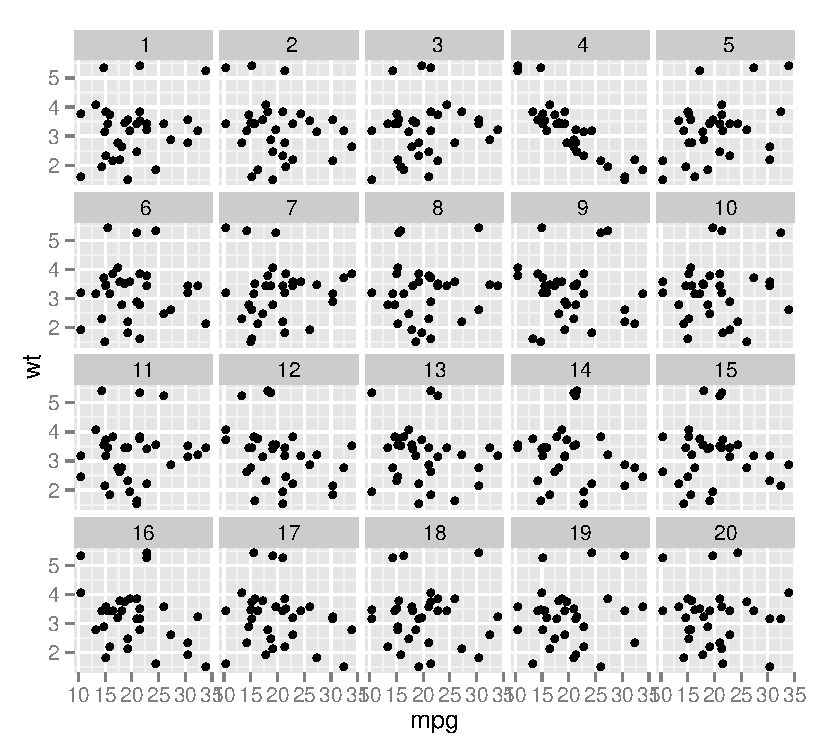
\includegraphics[scale=1]{nullabor-lineup.pdf}
\caption{A typical lineup. The plot of the actual data is embedded in a set of null plots which are generated assuming that the null hypothesis is true. The variable ``mpg'' is permuted 19 times to obtain the 19 null plots. Can you identify the plot which has the steepest slope? The true position of the plot can be obtain by copying and pasting ``decrypt(...)'' from the output into R console.}
\label{lineup-ex}
\end{center}
\end{figure*}

\subsection{The Rorschach protocol}\label{the-rorschach-protocol}

The Rorschach protocol is used to calibrate the eyes for variation due
to sampling. The plots generated corresponds to the null datasets, data
that is consistent with a null hypothesis. The \texttt{"rorschach"}
function returns a set of null plots which are shown to observers to
calibrate their eyes with variation. Like the \texttt{"lineup"}
function, the null generating mechanism should be provided as an input
along with a real dataset. A probability can also be given as input
which dictates the chance of including the true data with null data.

\begin{verbatim}
> head(rorschach(null_permute("mpg"), mtcars, n = 8, p = 0), 20)

   .n  mpg cyl  disp  hp drat    wt  qsec vs am gear carb
1   1 17.3   6 160.0 110 3.90 2.620 16.46  0  1    4    4
2   1 32.4   6 160.0 110 3.90 2.875 17.02  0  1    4    4
3   1 21.0   4 108.0  93 3.85 2.320 18.61  1  1    4    1
4   1 21.0   6 258.0 110 3.08 3.215 19.44  1  0    3    1
5   1 15.5   8 360.0 175 3.15 3.440 17.02  0  0    3    2
6   1 30.4   6 225.0 105 2.76 3.460 20.22  1  0    3    1
7   1 14.7   8 360.0 245 3.21 3.570 15.84  0  0    3    4
8   1 22.8   4 146.7  62 3.69 3.190 20.00  1  0    4    2
9   1 15.0   4 140.8  95 3.92 3.150 22.90  1  0    4    2
10  1 19.2   6 167.6 123 3.92 3.440 18.30  1  0    4    4
11  1 22.8   6 167.6 123 3.92 3.440 18.90  1  0    4    4
12  1 18.7   8 275.8 180 3.07 4.070 17.40  0  0    3    3
13  1 26.0   8 275.8 180 3.07 3.730 17.60  0  0    3    3
14  1 15.2   8 275.8 180 3.07 3.780 18.00  0  0    3    3
15  1 21.4   8 472.0 205 2.93 5.250 17.98  0  0    3    4
16  1 24.4   8 460.0 215 3.00 5.424 17.82  0  0    3    4
17  1 21.5   8 440.0 230 3.23 5.345 17.42  0  0    3    4
18  1 19.7   4  78.7  66 4.08 2.200 19.47  1  1    4    1
19  1 15.2   4  75.7  52 4.93 1.615 18.52  1  1    4    2
20  1 21.4   4  71.1  65 4.22 1.835 19.90  1  1    4    1
\end{verbatim}

%\begin{Shaded}
%\begin{Highlighting}[]
%\KeywordTok{head}\NormalTok{(}\KeywordTok{rorschach}\NormalTok{(}\KeywordTok{null_permute}\NormalTok{(}\StringTok{"mpg"}\NormalTok{), mtcars, }\DataTypeTok{n =} \DecValTok{8}\NormalTok{, }\DataTypeTok{p =} \DecValTok{0}\NormalTok{), }\DecValTok{20}\NormalTok{)}
%\end{Highlighting}
%\end{Shaded}
%
%\begin{verbatim}
%##    .n  mpg cyl  disp  hp drat    wt  qsec vs am gear carb
%## 1   1 21.0   6 160.0 110 3.90 2.620 16.46  0  1    4    4
%## 2   1 15.5   6 160.0 110 3.90 2.875 17.02  0  1    4    4
%## 3   1 10.4   4 108.0  93 3.85 2.320 18.61  1  1    4    1
%## 4   1 19.2   6 258.0 110 3.08 3.215 19.44  1  0    3    1
%## 5   1 13.3   8 360.0 175 3.15 3.440 17.02  0  0    3    2
%## 6   1 15.0   6 225.0 105 2.76 3.460 20.22  1  0    3    1
%## 7   1 18.7   8 360.0 245 3.21 3.570 15.84  0  0    3    4
%## 8   1 10.4   4 146.7  62 3.69 3.190 20.00  1  0    4    2
%## 9   1 14.7   4 140.8  95 3.92 3.150 22.90  1  0    4    2
%## 10  1 15.2   6 167.6 123 3.92 3.440 18.30  1  0    4    4
%## 11  1 26.0   6 167.6 123 3.92 3.440 18.90  1  0    4    4
%## 12  1 21.5   8 275.8 180 3.07 4.070 17.40  0  0    3    3
%## 13  1 21.0   8 275.8 180 3.07 3.730 17.60  0  0    3    3
%## 14  1 17.8   8 275.8 180 3.07 3.780 18.00  0  0    3    3
%## 15  1 17.3   8 472.0 205 2.93 5.250 17.98  0  0    3    4
%## 16  1 14.3   8 460.0 215 3.00 5.424 17.82  0  0    3    4
%## 17  1 18.1   8 440.0 230 3.23 5.345 17.42  0  0    3    4
%## 18  1 22.8   4  78.7  66 4.08 2.200 19.47  1  1    4    1
%## 19  1 16.4   4  75.7  52 4.93 1.615 18.52  1  1    4    2
%## 20  1 19.2   4  71.1  65 4.22 1.835 19.90  1  1    4    1
%\end{verbatim}

\begin{verbatim}
> qplot(mpg, wt, data = rorschach(null_permute("mpg"), mtcars, n = 9, p = 0)) 
+ facet_wrap(~ .n)
\end{verbatim}

\begin{figure*}[hbtp]
\begin{center}
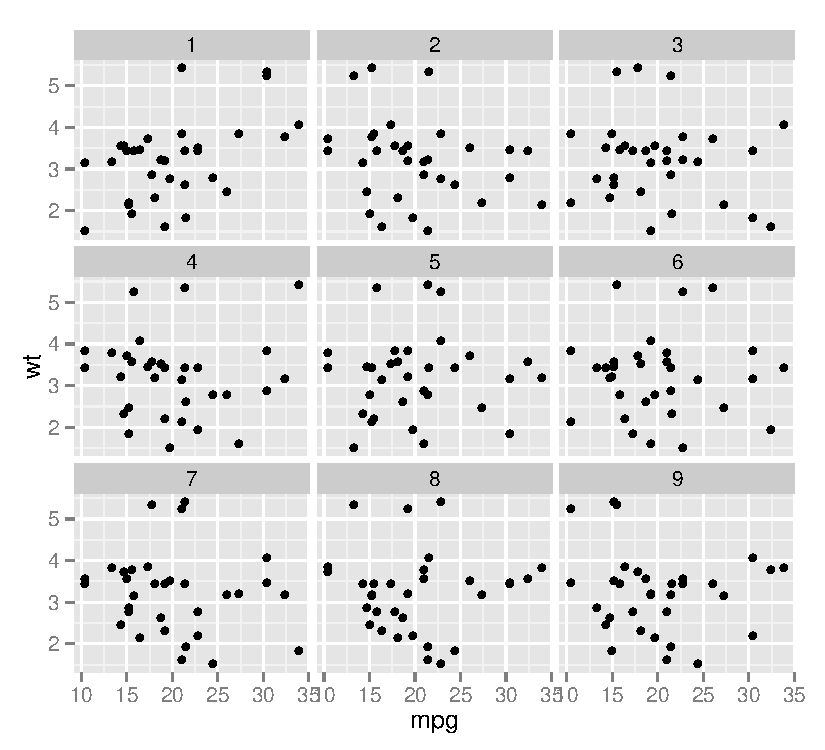
\includegraphics[scale=1]{nullabor-rorschach.pdf}
\caption{Illustration of the Rorschach protocol. These nine scatterplots are obtained by permuting the variable ``mpg'' while keeping the variable ``wt'' fixed. Does it look like the strength of the relationship is same in all the plots? Is there a plot which has more interesting pattern than others? }
\label{rorschach}
\end{center}
\end{figure*}

The Rorschach protocol helps us to calibrate our vision to the natural variability in plots in which the data is generated from scenarios consistent with the null hypothesis. Figure \ref{rorschach} is drawn using the rorschach data using package \textbf{ggplot2}. Can we identify any interesting pattern in the plots? Is there a plot among these which has a stronger structure than others?

\section{Distance metrics}\label{distance-metrics}

There are five different distance metrics in \textbf{nullabor} package,
named \texttt{"bin\_dist"}, \texttt{"box\_dist"}, \texttt{"reg\_dist"},
\texttt{"sep\_dist"} and \texttt{"uni\_dist"}. The different distance
metrics are constructed so that they can identify the different
properties of the data. \texttt{"uni\_dist"} works for univariate data
while the others works for all types of bivariate data. Binned distance
is a generic distance which can be used in any situations while the
other distance metrics are constructed so that they can identify the
effect of graphical elements in a plot like an overlaid regression line
or presence of defined clusters. To calculate some of the metrics,
additional informations like a class variable or the number of bins
should be provided.

\subsection{Distance for univariate
data}\label{distance-for-univariate-data}

\texttt{"uni\_dist"} is a distance metric which calculates the euclidean
distance between the first four central moments of two univariate data.
A typical usage would be when one needs to calculate the distance
between the two histograms drawn from two datasets.

%\begin{Shaded}
%\begin{Highlighting}[]
%\KeywordTok{library}\NormalTok{(nullabor)}
%\KeywordTok{uni_dist}\NormalTok{(}\KeywordTok{rnorm}\NormalTok{(}\DecValTok{100}\NormalTok{), }\KeywordTok{rpois}\NormalTok{(}\DecValTok{100}\NormalTok{, }\DecValTok{2}\NormalTok{))}
%\end{Highlighting}
%\end{Shaded}
%
%\begin{verbatim}
%## [1] 2.309
%\end{verbatim}

\begin{verbatim}
> uni_dist(X = rnorm(100), PX = rpois(100, 2))

[1] 2.980522
\end{verbatim}

\subsection{Distance based on regression
parameters}\label{distance-based-on-regression-parameters}

\texttt{"reg\_dist"} is a distance metric which calculates the euclidean
distance between the regression parameters of a model fitted to one plot
and that of another plot. It is advisable to use this distance in
situations where a regression line is overlaid on a scatterplot.

%\begin{Shaded}
%\begin{Highlighting}[]
%\KeywordTok{with}\NormalTok{(mtcars, }\KeywordTok{reg_dist}\NormalTok{(}\KeywordTok{data.frame}\NormalTok{(wt, mpg), }\KeywordTok{data.frame}\NormalTok{(}\KeywordTok{sample}\NormalTok{(wt), mpg)))}
%\end{Highlighting}
%\end{Shaded}
%
%\begin{verbatim}
%## [1] 618.1
%\end{verbatim}

\begin{verbatim}
> X <- data.frame(X1 = mtcars$wt, X2 = mtcars$mpg)
> PX <- data.frame(X1 = sample(mtcars$wt), X2 = mtcars$mpg)
> reg_dist(X, PX)

[1] 132.9617
\end{verbatim}

\subsection{Distance based on
boxplots}\label{distance-based-on-boxplots}

\texttt{"box\_dist"} is a distance metric which works for side-by-side
boxplots with two levels. The first quartile, median and the third
quartile are calculated for each box and the absolute distances of these
are calculated for the two boxes. \texttt{"box\_dist"} calculates the
euclidean distance between these absolute distances for the two plots.
The boxplot distance should be used in situations where a side-by-side
boxplot is used to compare the distribution of a variable at two
different levels.

%\begin{Shaded}
%\begin{Highlighting}[]
%\KeywordTok{with}\NormalTok{(mtcars, }\KeywordTok{box_dist}\NormalTok{(}\KeywordTok{data.frame}\NormalTok{(}\KeywordTok{as.factor}\NormalTok{(am), mpg),  } \\
%\KeywordTok{data.frame}\NormalTok{(}\KeywordTok{as.factor}\NormalTok{(}\KeywordTok{sample}\NormalTok{(am)), mpg)))}
%\end{Highlighting}
%\end{Shaded}
%
%\begin{verbatim}
%## [1] 11.81
%\end{verbatim}

\begin{verbatim}
> X <- data.frame(X1 = as.factor(mtcars$am), X2 = mtcars$mpg)
> PX <- data.frame(X1 = as.factor(sample(mtcars$am)), X2 = mtcars$mpg)
> box_dist(X, PX)

[1] 12.94846
\end{verbatim}

\subsection{Distance based on
separation}\label{distance-based-on-separation}

\texttt{"sep\_dist"} is a distance metric based on the separation
between clusters. The separation between clusters is defined by the
minimum distances of a point in the cluster to a point in another
cluster. The separation between the clusters for a given dataset is
calculated. An euclidean distance is calculated between the separation
for the given dataset and another dataset. The number of clusters in the
dataset should be provided. If not, the hierarchical clustering method
is used to obtain the clusters.

%\begin{Shaded}
%\begin{Highlighting}[]
%\KeywordTok{with}\NormalTok{(mtcars, }\KeywordTok{sep_dist}\NormalTok{(}\KeywordTok{data.frame}\NormalTok{(wt, mpg,  }\KeywordTok{as.numeric}\NormalTok{(}\KeywordTok{as.factor}\NormalTok{(mtcars$cyl))), }\\
%\KeywordTok{data.frame}\NormalTok{(}\KeywordTok{sample}\NormalTok{(wt), mpg,  }\KeywordTok{as.numeric}\NormalTok{(}\KeywordTok{as.factor}\NormalTok{(mtcars$cyl))), }\DataTypeTok{nclust =} \DecValTok{3}\NormalTok{))}
%\end{Highlighting}
%\end{Shaded}
%
%\begin{verbatim}
%## [1] 0.01651
%\end{verbatim}

\begin{verbatim}
> X <- data.frame(X1 = mtcars$wt, X2 = mtcars$mpg, 
cl = as.numeric(as.factor(mtcars$cyl)))
> PX <- data.frame(X1 = sample(mtcars$wt), X2 = mtcars$mpg, 
cl = as.numeric(as.factor(mtcars$cyl)))
> sep_dist(X, PX, clustering = TRUE)

[1] 0.2552364

> sep_dist(X, PX, clustering = FALSE, nclust = 3)

[1] 0.04571194
\end{verbatim}

\subsection{Binned Distance}\label{binned-distance}

\texttt{"bin\_dist"} is a generic distance which works for any situation
for any dataset. For a given bivariate dataset, X and Y variables are
divided into p and q bins respectively to obtain pq cells. The number of
points falling in each cell are counted for a given dataset.
\texttt{"bin\_dist"} between two datasets calculates the euclidean
distance between the cell counts of these two data. The values of p and
q should be provided as arguments.

%\begin{Shaded}
%\begin{Highlighting}[]
%\KeywordTok{with}\NormalTok{(mtcars, }\KeywordTok{bin_dist}\NormalTok{(}\KeywordTok{data.frame}\NormalTok{(wt, mpg), } \\
%\KeywordTok{data.frame}\NormalTok{(}\KeywordTok{sample}\NormalTok{(wt), mpg), }\DataTypeTok{lineup.dat =} \OtherTok{NULL}\NormalTok{, }\DataTypeTok{X.bin =} \DecValTok{5}\NormalTok{, }\DataTypeTok{Y.bin =} \DecValTok{5}\NormalTok{))}
%\end{Highlighting}
%\end{Shaded}
%
%\begin{verbatim}
%## [1] 8.718
%\end{verbatim}

\begin{verbatim}
> X <- data.frame(X1 = mtcars$wt, X2 = mtcars$mpg)
> PX <- data.frame(X1 = sample(mtcars$wt), X2 = mtcars$mpg)
> bin_dist(X,PX, lineup.dat = NULL, X.bin = 5, Y.bin = 5)

[1] 7.745967
\end{verbatim}

\section{Calculation of mean distances and difference}

\subsection{Calculating the mean distances for the plots in the
lineup}\label{calculating-the-mean-distances-for-the-plots-in-the-lineup}

It is interesting to see whether the true plot in a lineup is different
from all the null plots. To find this the distances between the true
plot and all the null plots are calculated and the mean of these
distances is calculated. Similarly, for each null plot, the distance
between the null plot and all the other null plots is calculated and
averaged to obtain the mean distance for each null plot.
\texttt{"calc\_mean\_dist"} calculates the mean distance corresponding
to each plot in the lineup. If the mean distance of the true plot is
larger than the mean distances of all the null plots, the lineup is
considered easy. If one of the null plots has a larger mean distance
than the true plot, the lineup is considered difficult.

\begin{figure*}[hbtp]
\begin{center}
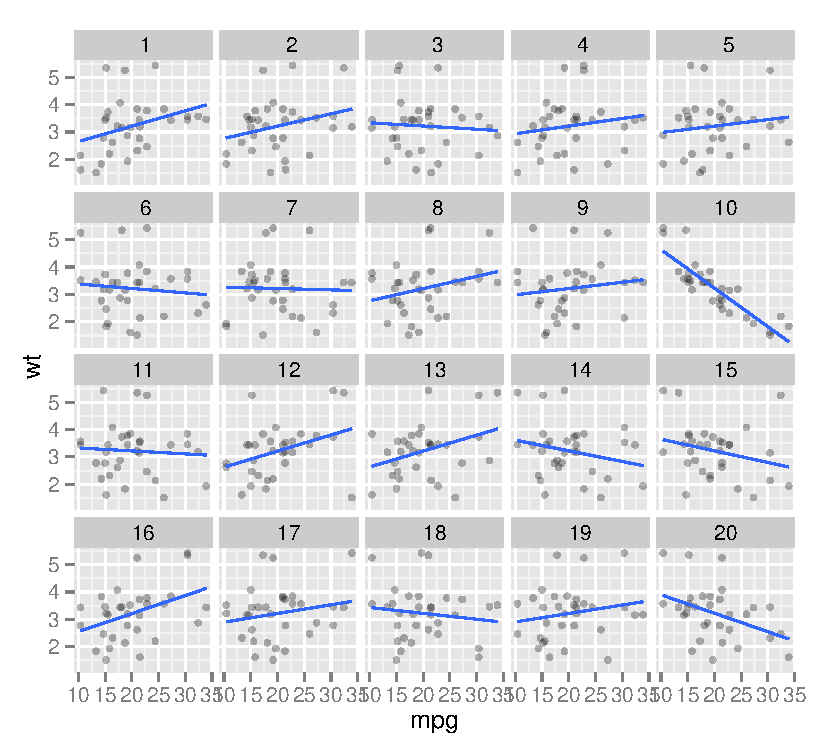
\includegraphics[scale=1.2]{nullabor-reg-ex.pdf}
\caption{Lineup plot of size $m = 20$ of scatterplots between ``mpg'' and ``wt'' with a regression line overlaid. The plot of the actual data is randomly placed among the set of null plots. The position of the plot of the actual data is 10. }
\label{lineup-reg}
\end{center}
\end{figure*}

%\begin{Shaded}
%\begin{Highlighting}[]
%\KeywordTok{library}\NormalTok{(dplyr)}
%\KeywordTok{calc_mean_dist}\NormalTok{(}\KeywordTok{lineup}\NormalTok{(}\KeywordTok{null_permute}\NormalTok{(}\StringTok{'mpg'}\NormalTok{), mtcars, }\DataTypeTok{pos =} \DecValTok{10}\NormalTok{), }\\
%\DataTypeTok{var =} \KeywordTok{c}\NormalTok{(}\StringTok{'mpg'}\NormalTok{, }\StringTok{'wt'}\NormalTok{), }\DataTypeTok{met =} \StringTok{'reg_dist'}\NormalTok{, }\DataTypeTok{pos =} \DecValTok{10}\NormalTok{)}
%\end{Highlighting}
%\end{Shaded}
%
%\begin{verbatim}
%## Source: local data frame [20 x 2]
%## 
%##    plotno mean.dist
%## 1       1    0.3030
%## 2       2    0.3923
%## 3       3    0.7187
%## 4       4    0.3150
%## 5       5    1.1514
%## 6       6    0.2730
%## 7       7    0.2857
%## 8       8    0.8783
%## 9       9    0.3466
%## 10     10    9.1644
%## 11     11    0.6400
%## 12     12    0.4516
%## 13     13    0.2748
%## 14     14    0.3411
%## 15     15    0.3779
%## 16     16    0.2864
%## 17     17    0.3057
%## 18     18    0.2761
%## 19     19    2.3577
%## 20     20    0.3885
%\end{verbatim}

\begin{verbatim}
> lineup.dat <- lineup(null_permute('mpg'), mtcars, pos = 10)
> calc_mean_dist(lineup.dat, var = c('mpg', 'wt'), met = 'reg_dist', pos = 10)
Source: local data frame [20 x 2]

   plotno  mean.dist
1       1  1.4105848
2       2  1.0551943
3       3  0.8912037
4       4  0.7146171
5       5  0.6708689
6       6  0.9966672
7       7  0.7674444
8       8  1.0456351
9       9  0.6642878
10     10 10.1982236
11     11  0.8703412
12     12  1.5049771
13     13  1.4878584
14     14  1.7874604
15     15  1.9487011
16     16  1.8179699
17     17  0.7709551
18     18  1.1412758
19     19  0.7568216
20     20  3.4081131
\end{verbatim}

\subsection{Calculating difference measure for
lineups}\label{calculating-difference-measure-for-lineups}

The mean distances for each plot in the lineup are obtained using
\texttt{"calc\_mean\_dist"}.\texttt{"calc\_diff"} calculates the
difference between the mean distance for the true plot and the maximum
mean distance for the null plots.

%\begin{Shaded}
%\begin{Highlighting}[]
%\KeywordTok{calc_diff}\NormalTok{(}\KeywordTok{lineup}\NormalTok{(}\KeywordTok{null_permute}\NormalTok{(}\StringTok{'mpg'}\NormalTok{), mtcars, }\DataTypeTok{pos =} \DecValTok{10}\NormalTok{), }\DataTypeTok{var =} \KeywordTok{c}\NormalTok{(}\StringTok{'mpg'}\NormalTok{, }\StringTok{'wt'}\NormalTok{), } \\
%\DataTypeTok{met =} \StringTok{'reg_dist'}\NormalTok{, }\DataTypeTok{dist.arg =} \OtherTok{NULL}\NormalTok{, }\DataTypeTok{pos =} \DecValTok{10}\NormalTok{)}
%\end{Highlighting}
%\end{Shaded}
%
%\begin{verbatim}
%## [1] 6.637
%\end{verbatim}

\begin{verbatim}
> calc_diff(lineup.dat, var = c('mpg', 'wt'), met = 'reg_dist', dist.arg = NULL, 
pos = 10)

[1] 6.79011
\end{verbatim}


\section{Selection of bins}\label{select-bins}

Binned distance is highly affected by the choice of the number of bins.
The number of bins is provided by the user and this can be subjective.
This motivates to design a way to select the optimum number of bins to
be used. \texttt{"opt\_diff"} finds the optimal number of bins in both x
and y direction which should be used to calculate the binned distance.
The binned distance is calculated for each combination of provided
choices of number of bins in x and y direction and finds the difference
using \texttt{"calc\_diff"} for each combination. The combination for
which the difference is maximum should be used.

%\begin{Shaded}
%\begin{Highlighting}[]
%\KeywordTok{library}\NormalTok{(ggplot2)}
%\NormalTok{opt.diff <-}\StringTok{ }\KeywordTok{opt_bin_diff}\NormalTok{(}\KeywordTok{lineup}\NormalTok{(}\KeywordTok{null_permute}\NormalTok{(}\StringTok{'mpg'}\NormalTok{), mtcars, }\DataTypeTok{pos =} \DecValTok{10}\NormalTok{), }\DataTypeTok{var =} \KeywordTok{c}\NormalTok{(}\StringTok{'mpg'}\NormalTok{, }\StringTok{'wt'}\NormalTok{), }\DecValTok{2}\NormalTok{, }\DecValTok{10}\NormalTok{, }\DecValTok{2}\NormalTok{, }\DecValTok{10}\NormalTok{, }\DataTypeTok{pos =} \DecValTok{10}\NormalTok{, }\DataTypeTok{plot =} \OtherTok{TRUE}\NormalTok{)}
%\KeywordTok{head}\NormalTok{(opt.diff$dat)}
%\end{Highlighting}
%\end{Shaded}
%
%\begin{verbatim}
%## Source: local data frame [6 x 3]
%## Groups: xbins
%## 
%##   xbins ybins    Diff
%## 1     2     2 -1.1123
%## 2     2     3 -1.1023
%## 3     2     4 -0.7199
%## 4     2     5 -0.7199
%## 5     2     6 -1.3007
%## 6     2     7 -0.7199
%\end{verbatim}
%
%\begin{Shaded}
%\begin{Highlighting}[]
%\NormalTok{opt.diff$p}
%\end{Highlighting}
%\end{Shaded}

\begin{verbatim}
> opt.diff <- opt_bin_diff(lineup.dat, var = c('mpg', 'wt'), 2, 10, 2, 10, pos = 10, 
plot = TRUE)
> head(opt.diff$dat)

Source: local data frame [6 x 3]
Groups: xbins

  xbins ybins       Diff
1     2     2 -0.1033782
2     2     3 -0.7769468
3     2     4 -0.4836467
4     2     5 -0.4836467
5     2     6 -0.4956530
6     2     7 -0.4836467

> opt.diff$p
\end{verbatim}

\begin{figure*}[hbtp]
\begin{center}
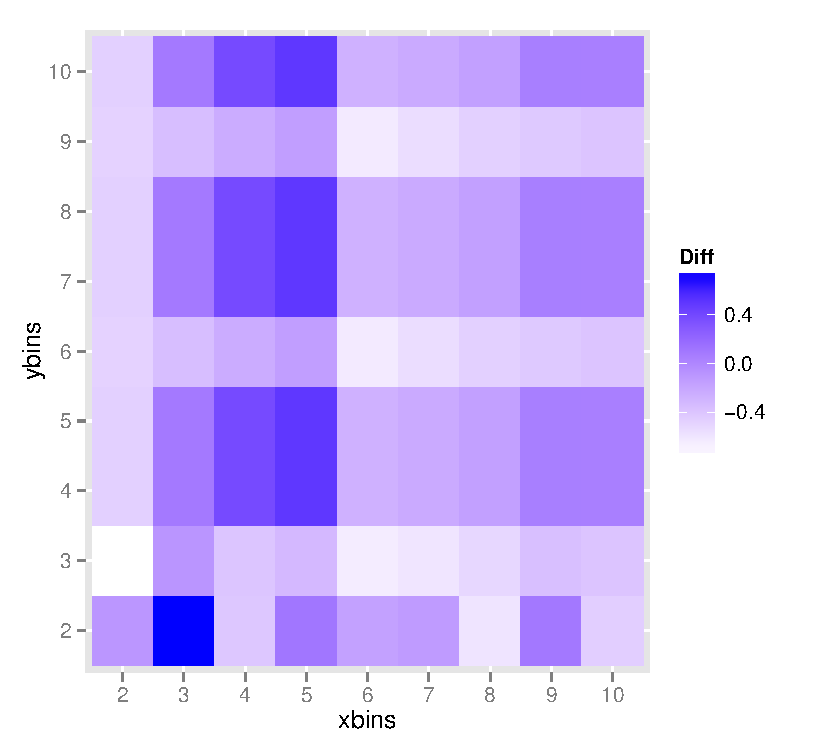
\includegraphics[scale=0.7]{nullabor-opt-bin.pdf}
\caption{Illustration of the optimum bin selection procedure. The obtained lineup data from subsection \ref{calculating-the-mean-distances-for-the-plots-in-the-lineup} is used to generate difference between the true plot and the maximum of the null plots using a binned distance for all combinations of number of bins on both x and y axes. The number of bins on x and y axes are plotted on x and y respectively with the colors showing the differences. The darker color represents larger difference. }
\label{opt-bin}
\end{center}
\end{figure*}

\section{Distribution of distance metrics}\label{distr}

\subsection{Empirical distribution of distance
metrics}\label{distribution-of-distance-metrics}

Measuring the quality of a lineup is interesting. But it may also be
important to compare a few lineups. \texttt{"distmet"} function provides
the empirical distribution of the distance metrics based on the mean
distance of the true plot and the mean distance from the null plots. The
lineup data, the null generating mechanism and the choice of the
distance metric has to be provided. Users have the flexibility of using
their distance metrics. The position of the true plot in the lineup has
to be provided as well. If the distance metrics require additional
arguments, those have to be provided as well.

%\begin{Shaded}
%\begin{Highlighting}[]
%\KeywordTok{library}\NormalTok{(ggplot2)}
%\NormalTok{lineup.dat <-}\StringTok{ }\KeywordTok{lineup}\NormalTok{(}\KeywordTok{null_permute}\NormalTok{(}\StringTok{'mpg'}\NormalTok{), mtcars, }\DataTypeTok{pos =} \DecValTok{10}\NormalTok{)}
%\KeywordTok{qplot}\NormalTok{(mpg, wt, }\DataTypeTok{data =} \NormalTok{lineup.dat, }\DataTypeTok{geom =} \StringTok{'point'}\NormalTok{) +}\StringTok{ }\KeywordTok{facet_wrap}\NormalTok{(~}\StringTok{ }\NormalTok{.sample)}
%\end{Highlighting}
%\end{Shaded}
%
%Copy and paste the output of lineup.dat to get the position of the true
%plot
%
%\begin{Shaded}
%\begin{Highlighting}[]
%\CommentTok{#decrypt('...') }
%\CommentTok{#[1] 'True data in position 10' # Use pos = 10}
%\end{Highlighting}
%\end{Shaded}

%\begin{figure*}[hbtp]
%\begin{center}
%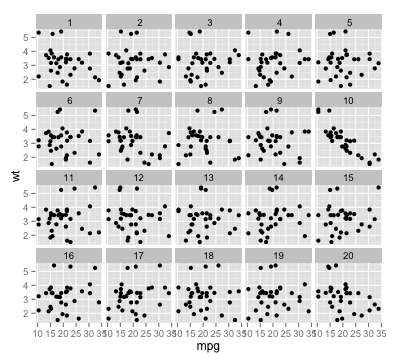
\includegraphics[scale=0.75]{unnamed-chunk-15.png}
%\end{center}
%\end{figure*}
%
%\begin{Shaded}
%\begin{Highlighting}[]
%\KeywordTok{library}\NormalTok{(dplyr)}
%\NormalTok{dist.vals <-}\StringTok{ }\KeywordTok{distmet}\NormalTok{(lineup.dat, }\DataTypeTok{var =} \KeywordTok{c}\NormalTok{(}\StringTok{'mpg'}\NormalTok{, }\StringTok{'wt'}\NormalTok{),}\StringTok{'reg_dist'}\NormalTok{, }\KeywordTok{null_permute}\NormalTok{(}\StringTok{'mpg'}\NormalTok{), }\\
%\DataTypeTok{pos =} \DecValTok{10}\NormalTok{, }\DataTypeTok{repl =} \DecValTok{100}\NormalTok{, }\DataTypeTok{dist.arg =} \OtherTok{NULL}\NormalTok{) }
%\end{Highlighting}
%\end{Shaded}
%
%\begin{Shaded}
%\begin{Highlighting}[]
%\KeywordTok{head}\NormalTok{(dist.vals$lineup)}
%\end{Highlighting}
%\end{Shaded}
%
%\begin{verbatim}
%## Source: local data frame [6 x 2]
%## 
%##   plotno mean.dist
%## 1      1    1.2397
%## 2      2    0.3427
%## 3      3    0.3852
%## 4      4    0.6395
%## 5      5    0.3387
%## 6      6    0.3394
%\end{verbatim}
%
%\begin{Shaded}
%\begin{Highlighting}[]
%\NormalTok{dist.vals$diff}
%\end{Highlighting}
%\end{Shaded}
%
%\begin{verbatim}
%## [1] 6.119
%\end{verbatim}
%
%\begin{Shaded}
%\begin{Highlighting}[]
%\KeywordTok{head}\NormalTok{(dist.vals$closest)}
%\end{Highlighting}
%\end{Shaded}
%
%\begin{verbatim}
%## [1] 20  1  7 17 16
%\end{verbatim}
%
%\begin{Shaded}
%\begin{Highlighting}[]
%\KeywordTok{head}\NormalTok{(dist.vals$null_values)}
%\end{Highlighting}
%\end{Shaded}
%
%\begin{verbatim}
%## [1] 0.6358 0.5557 0.3349 1.2700 0.4673 0.3292
%\end{verbatim}
%
%\begin{Shaded}
%\begin{Highlighting}[]
%\NormalTok{dist.vals$pos}
%\end{Highlighting}
%\end{Shaded}
%
%\begin{verbatim}
%## [1] 10
%\end{verbatim}

\begin{verbatim}
> dist.vals1 <- distmet(lineup.dat, var = c('mpg', 'wt'),'reg_dist', null_permute('mpg'), 
pos = 10,  repl = 1000, dist.arg = NULL)
> head(dist.vals1$lineup)

Source: local data frame [6 x 2]

  plotno mean.dist
1      1 1.4105848
2      2 1.0551943
3      3 0.8912037
4      4 0.7146171
5      5 0.6708689
6      6 0.9966672

> dist.vals1$diff

[1] 6.79011

> head(dist.vals1$closest)

[1] 20 15 16 14 12

> head(dist.vals1$null_values)

[1] 1.0564997 0.4444821 0.3020866 0.3106895 0.8703144 0.9713040

> dist.vals$pos
[1] 10

\end{verbatim}

%\begin{Shaded}
%\begin{Highlighting}[]
%\NormalTok{dist.vals <-}\StringTok{ }\KeywordTok{distmet}\NormalTok{(lineup.dat, }\DataTypeTok{var =} \KeywordTok{c}\NormalTok{(}\StringTok{'mpg'}\NormalTok{, }\StringTok{'wt'}\NormalTok{),}\StringTok{'bin_dist'}\NormalTok{, }\KeywordTok{null_permute}\NormalTok{(}\StringTok{'mpg'}\NormalTok{), } \\
%\DataTypeTok{pos =} \DecValTok{10}\NormalTok{, }\DataTypeTok{repl =} \DecValTok{100}\NormalTok{, }\DataTypeTok{dist.arg =} \KeywordTok{list}\NormalTok{(}\DataTypeTok{lineup.dat =} \NormalTok{lineup.dat, }\DataTypeTok{X.bin =} \DecValTok{5}\NormalTok{, }\DataTypeTok{Y.bin =} \DecValTok{5}\NormalTok{)) }
%\end{Highlighting}
%\end{Shaded}

\subsection{Plotting the empirical distribution of the distance
metric}\label{plotting-the-empirical-distribution-of-the-distance-metric}

\texttt{"distplot"} functions plots the empirical distribution of the
distance metric, given the output of \texttt{"distmet"} function. The
distribution is shown in grey along the distance for the true plot in
orange and the distances for the null plots in black.

%\begin{Shaded}
%\begin{Highlighting}[]
%\KeywordTok{distplot}\NormalTok{(dist.vals)}
%\end{Highlighting}
%\end{Shaded}
\newpage

\begin{verbatim}
> distplot(dist.vals1)
\end{verbatim}

\begin{figure*}[hbtp]
\begin{center}
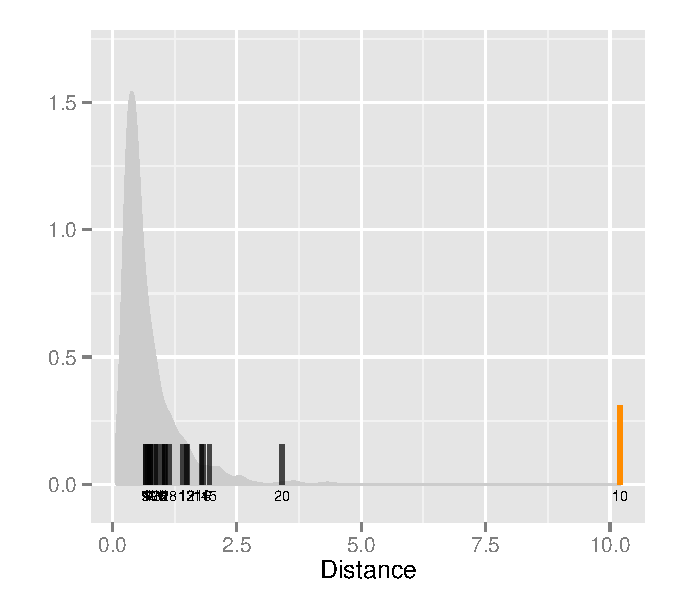
\includegraphics[scale=0.7]{nullabor-distr-reg.pdf}
\caption{Distribution of the \textbf{regression based distance} with the distance for the null plots of the lineup represented in black and the distance for the plot of the actual data represented by orange. The distance for the actual plot is much higher than the null plots and the actual plot can be easily identified as seen in Figure \ref{lineup-reg}. }
\label{dist-reg}
\end{center}
\end{figure*}

\newpage

\begin{verbatim}
> dist.vals2 <- distmet(lineup.dat, var = c('mpg', 'wt'), 'bin_dist', null_permute('mpg'), 
pos = 10, repl = 1000, dist.arg = list(lineup.dat = lineup.dat, X.bin = 6, Y.bin = 6))
> distplot(dist.vals2)
\end{verbatim}

\begin{figure*}[hbtp]
\begin{center}
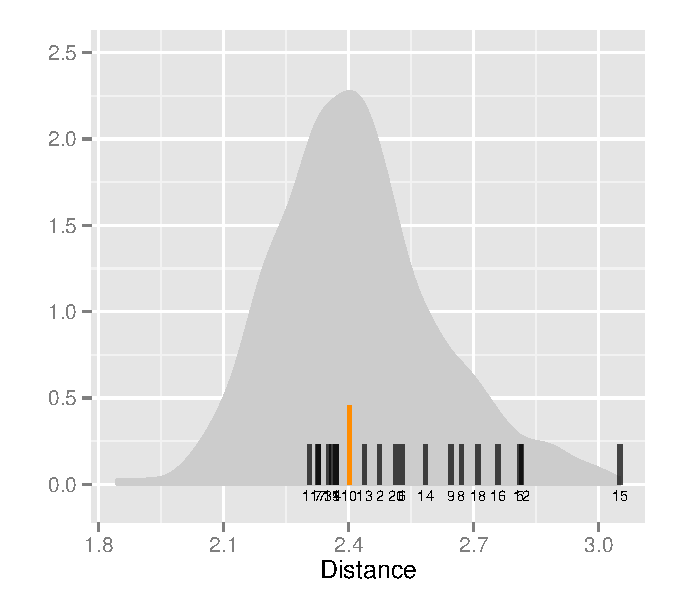
\includegraphics[scale=0.7]{nullabor-distr-bin-1.pdf}
\caption{Distribution of the \textbf{binned distance} with the distance for the null plots of the lineup represented in black and the distance for the plot of the actual data represented by orange. The number of bins used is 6 on both axes. The distance for the actual plot falls within the distances for the null plots. This shows that the lineup is difficult in the sense that the actual cannot be easily identified.  Hence the selection of the number of bins is important for binned distance. }
\label{dist-bin-1}
\end{center}
\end{figure*}

\newpage

\begin{verbatim}
> dist.vals3 <- distmet(lineup.dat, var = c('mpg', 'wt'), 'bin_dist', null_permute('mpg'), 
pos = 10, repl = 1000, dist.arg = list(lineup.dat = lineup.dat, X.bin = 3, Y.bin = 2))
> distplot(dist.vals3)
\end{verbatim}

\begin{figure*}[hbtp]
\begin{center}
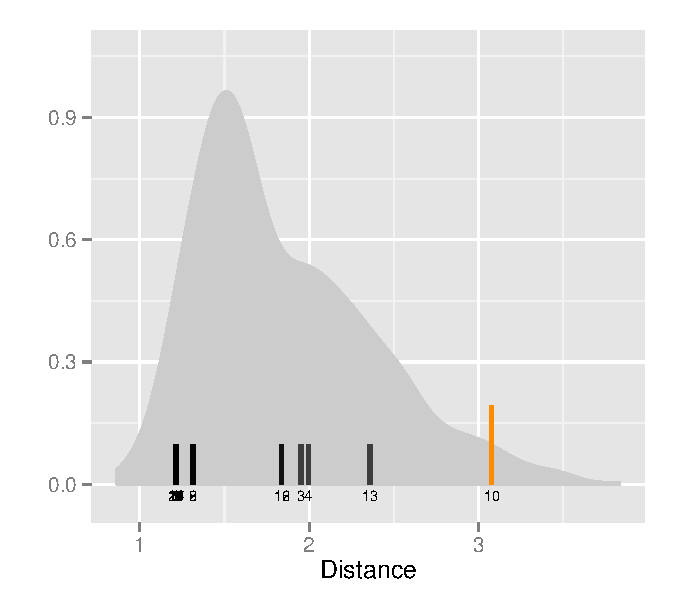
\includegraphics[scale=0.75]{nullabor-distr-bin-2.pdf}
\caption{Distribution of the \textbf{binned distance} with the distance for the null plots of the lineup represented in black and the distance for the plot of the actual data represented by orange. The number of bins used is 3 on x-axis and 2 on y-axis. The number of bins are selected by the optimal bin selection method using Figure \ref{opt-bin}. The distance for the actual plot is larger than the distances for the null plots which matches the lineup.}
\label{dist-bin-1}
\end{center}
\end{figure*}
